%!TeX root=../paper.tex

\section{Measuring Ambiguity}\label{sec:ambiguity}

Based on the expanded concept of path ambiguity introduced in the previous section, we propose a novel metric to evaluate ambiguity in bundled visualizations. Since bundling methods do not generate drawings from the original data, they operate on a given input drawing. Our metric aims to take the input drawing into account and incorporate the information from these spatial embeddings into the ambiguity calculation. To our knowledge, this is the only ambiguity metric that can compute ambiguity for both graph drawings and trail-sets, making it the first comprehensive path-ambiguity metric.

Our metric introduces two key contributions. First, we propose a spatially-aware approach that computes local ambiguity values throughout the drawing, providing detailed insight into problematic regions instead of reducing ambiguity to a single global value. Second, we introduce a continuous approach to crossing ambiguity that considers the similarity between overlapping paths, moving beyond the traditional binary classification of ambiguous crossings. These contributions enable a more nuanced evaluation of bundled visualizations while accounting for their spatial characteristics.

While the ambiguities presented in Edge-Path focus exclusively on edge bundling, they can be adapted to general path bundling. Edge-crossing ambiguities and path endpoint ambiguities remain unchanged, as they still introduce the same incorrect assumptions. Independent-edge ambiguities are also present, but instead of relying solely on individual vertices to trigger this ambiguity, we consider the spatial encodings of the endpoints; for example, by considering whether the vertices belong to the same cluster.

Next, we formalize these concepts into a metric that captures both the structural and spatial aspects of path ambiguity.

% ------- SUBSECTION -------

\subsection{Proposed metric}

Let $\mathcal{D}$ be the space of all possible drawings and $D(P) = \{p_i \subset \mathbb{R}^2 \}$ be a drawing of a path-set $P$, where $p_i$ can be either a straight line, for graph drawings, or a curve in space, for trail-sets. Let $B: \mathcal{D} \rightarrow \mathcal{D}$ be a general bundling operator, we formalize that a pair of paths $p_i \in D(P)$ and $B(p_j) \in B(D(P))$ as being counterparts of each other when $p_i$ generates $p_j$ after the bundling operator $B$ is applied to $D_G$. Finally, we define the metric as a scalar field $\omega : \mathbb{R}^2 \rightarrow \mathbb{R}_{+}$ that represents ambiguity throughout the drawing.

Before delving into the technical details, we present a high-level overview of $\omega$ formulation. First, we take all $B(p_i) \in B(D(P))$ that intersect a neighborhood and select their counterparts in $D(P)$. We then take the average distance between all possible pairs of the selected paths. Additionally, we apply both a convolution and a normalization steps to the scalar field to smooth the resulting values. 

We argue that the comparison between paths in $B(D(P))$ and their original counterparts in $D(P)$ bridges the gap between both drawings, providing an estimate of bundle formation quality throughout the bundled drawing. We now present how $\omega$ is defined for a given location $\mathbf{x} \in \mathbb{R}^2$, detailing each step of its calculation: (1) the selection of paths and their counterparts, (2) the distance calculations between paths, (3) the convolution, and (4) the normalization process.

% --- step 1:

\textbf{Selection of paths and counterparts (step 1):}
% lucas: I was naming the two user defined parameters with rho for consistency and easy identification of parameters vs constants, but it following the email I changed it to simply r, m, and c.
The first step involves selecting the paths from $B(D(P))$ that affect ambiguity at point $\mathbf{x} \in \mathbb{R}^2$. Given a user-defined parameter $r \in \mathbb{N}$, we identify all paths $B(p_i) \in B(D(P)), B(p_i) \cap N_r(\mathbf{x}) \neq \varnothing$, that intersect a neighborhood $N_r(\mathbf{x})$ of radius $r$ and center $\mathbf{x}$. For each intersecting path, we collect the corresponding counterparts from $D(P)$ and group them in the set $\bar{P}_{\mathbf{x}} \in D(P)$.

% --- step 2:

\textbf{Path distances calculation (step 2):}
With the set $\bar{P}_p$ defined, we take the average of the distances between all pairs in $\bar{P}_p$. We define a distance function $\lambda : D(P) \times D(P) \rightarrow \mathbb{R}_{+}$ as a modified weak \emph{Fr\'echet distance}. Let $| p_i |$ be the cardinality of $p_i \in D(P)$, $\| p_i - p_j \|$ be the Euclidean distance between $p_i, p_j \in D(P)$, and $T : \mathbb{R}^2 \rightarrow \mathbb{R}^2$ be a function that returns the tangent of $p_i \in D(P)$ at a given point $\mathbf{a} \in p_i$, we define $\lambda$ defined as follows:

% lucas: if I got the email right, the denominator there is wrong. In the discrete version, we do not divide by the length of the curve, we divide by the number of control point inside it. That is, if we have n sample distances from a to b, we divide the sum of the distances by n. So, I believe here we should divide by the cardinality of p_i here, but I might be completely off.
\begin{equation}
\lambda(p_i, p_j) =
\bigintsss_{\mathbf{a} \in p_i} \frac
{\displaystyle \min_{\mathbf{b} \in p_j} \big(\| \mathbf{a} - \mathbf{b} \|\big) \big(T(\mathbf{a}) \cdot T(\mathbf{b})\big)^2}
{|p_i|}
ds
\end{equation}

By swapping the minimum ``leash'' from the weak \emph{fr\'echet distance}, we make the function less susceptible to drastic changes from outliers. Taking the case depicted in Figure \ref{fig:frechet_example}, the two paths are similar to each other but have a small detour in the middle. With the weak \emph{fr\'echet distance}, this detour drastically alters the resulting distance. However, since these paths share similar endpoints and roughly the same shape, a smaller distance is more desirable. By taking the average, we successfully achieve this, making $\lambda$ better suited for our needs.

\begin{figure}[ht]
\centering
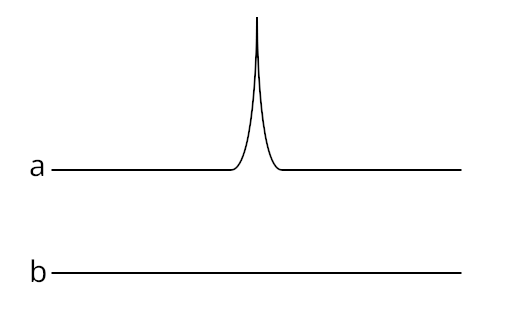
\includegraphics[width=0.48\linewidth]{frechet-example.png}
\caption{Example of case where the weak \emph{fr\'echet distance} is not ideal.}
\label{fig:frechet_example}
\end{figure}

Another critical aspect is the square of the dot product between the tangents of $p_i, p_j \in D(P)$. This dot product reduces the contribution of paths that intersect at near-perpendicular angles, aligning with the edge-crossing ambiguity principle discussed earlier. Squaring the term ensures smooth, differentiable modulation while preventing negative values, preserving the stability and interpretability of $\lambda$.

The distance function $\lambda$ is the core of $\omega$; however, only using the average of distances may generate undesirable results in some datasets. To avoid any issues, we can modulate $\lambda$ with user-defined parameters. We define two functions to modulate $\lambda$ based on the distance from the endpoints of the path and the distance of the path from $\mathbf{x}$. Next, we discuss both the issues that may arise and the modulating functions themselves.

% - distance from endpoints:

\emph{Modulating by distance from endpoints:}
Vertex-adjacent regions in graph drawings often exhibit a higher path density, as multiple paths originate from or terminate at these regions. This concentration leads to large $\bar{P}_{\mathbf{x}}$ sets at those regions and, in certain datasets, results in ambiguity being disproportionately concentrated in vertex clusters. Figure \ref{fig:imbalance_problem} exemplifies this pattern, with ambiguity color-coded from blue to red in increasing ambiguity values. However, we argue that the most problematic regions for path ambiguity tend to be along the middle sections of paths, rather than at their endpoints, since these areas lack the inherent structural context provided by the endpoints.

\begin{figure}[ht]
\centering
\subfloat[$\lambda$ without modulation.]{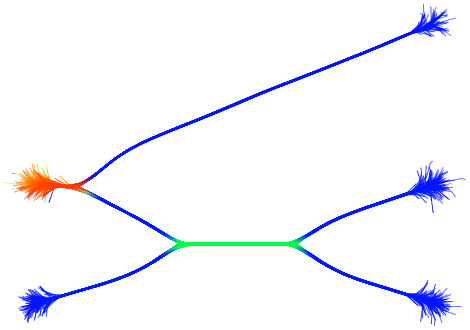
\includegraphics[width=0.48\linewidth]{imbalance-problem.png}\label{fig:imbalance_problem}}
\subfloat[$\lambda$ with $\beta$ modulation.]{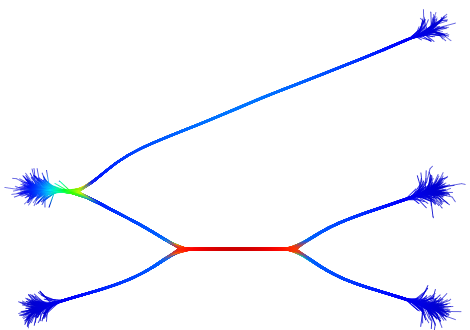
\includegraphics[width=0.48\linewidth]{imbalance-solution.png}\label{fig:imbalance_solution}}\\
\caption{Example of ambiguity concentration on endpoints of $\lambda$, with (b) and without (a) $\beta$ modulation.}
\end{figure}

% lucas: there is probably a more elegant way to describe this, but I couldn't figure it out.
To address this issue, we introduce a modulation function $\beta_{\mathbf{x}} : B(D(P)) \rightarrow [0, 1]$ that weights each path's ambiguity contribution based on its position relative to endpoints. Given a user-defined parameter $m \in [0, \frac{1}{2}[$, $\beta_{\mathbf{x}}$ smoothly transitions from zero near the endpoints to its maximum value in the interval $[m, 1 - m]$. The function uses the normalized arc-length parameter of $B(p_i) \in B(D(P))$ that is closest to $\mathbf{x}$. While the specific formulation of $\beta_{\mathbf{x}}$ is flexible, it should follow the general shape shown in Figure \ref{fig:beta}, where the x-axis represents the normalized position along the path.

\begin{figure}[ht]
\begin{tikzpicture}[scale=1.0]
\begin{axis}[
    axis x line=center,
    axis y line=center,
    x label style={at={(axis description cs:.5,-0.05)},anchor=north},
    y label style={at={(axis description cs:-0.1,.5)},rotate=90,anchor=south},
    xlabel = {Normalized arc-length parameter.},
    ylabel = {$\beta_{\mathbf{x}}$},
    xtick={0},
    ytick={0, 0.5, 1.0},
    xmin=-0.1, xmax=4.6,
    ymin=-0.15, ymax=1.1,
]

\addplot [red, domain=0:1.2  ] { 0.5 - (cos(x         * 48 * pi) / 2) }; 
\addplot [red, domain=1.2:2.8] {  1 };           
\addplot [red, domain=2.8:4  ] { 0.5 - (cos((x - 1.6) * 48 * pi) / 2) }; 

\draw [dashed] (axis cs:1.2,\pgfkeysvalueof{/pgfplots/ymin}) -- (axis cs:1.2,\pgfkeysvalueof{/pgfplots/ymax});
\draw [thick, <->] (axis cs:0,-0.05) -- (axis cs:1.2,-0.05) node[pos=0.5, below] {$m$};

\draw [dashed] (axis cs:2.8,\pgfkeysvalueof{/pgfplots/ymin}) -- (axis cs:2.8,\pgfkeysvalueof{/pgfplots/ymax});
\draw [thick, <->] (axis cs:2.8,-0.05) -- (axis cs:4,-0.05) node[pos=0.5, below] {$m$};

\end{axis}
\end{tikzpicture}
\caption{Graph with the expected shape of $\beta_{\mathbf{x}}$.}
\label{fig:beta}
\end{figure}

We can see the results of applying the $\beta_p$ function in Figure \ref{fig:imbalance_solution}. The modulation effectively shifts the focus of ambiguity from the vertex-adjacent regions to the middle sections of the paths, as intended. This redistribution of ambiguity aligns with our earlier assertion that the most problematic regions typically occur along the middle of path paths rather than at their endpoints.

% - distance from x:

\emph{Modulating by distance from $\mathbf{x}$}:
Another issue present in the initial $\lambda$ formulation is the discontinuity in the scalar field. Using $\mathbf{x}$ as a reference point, as paths approach $N_r(\mathbf{x})$, their proximity is not captured by $\lambda$; when these approaching paths start to intersect $N_r(\mathbf{x})$, they are then included in $\bar{P}_{\mathbf{x}}$ with full weight. This abrupt change in the calculation of $\lambda$ creates discontinuities in the scalar field at the neighborhood's boundary. This is exemplified in Figure \ref{fig:linearity_problem}, where the ambiguity sharply transitions from low (blue) to high (red) in the central region.

\begin{figure}[ht]
\centering
\subfloat[$\lambda$ without modulation.]{
    \begin{tikzpicture}[spy using outlines={circle,red,magnification=3.5,size=2.5cm, connect spies}]
    \node {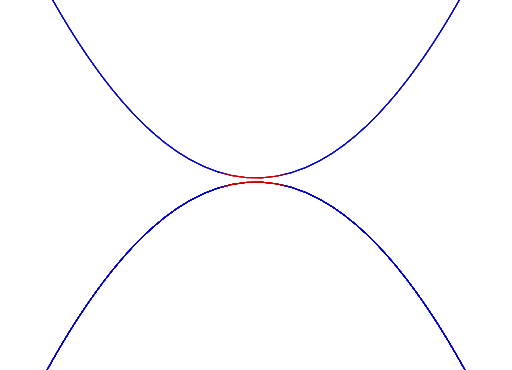
\includegraphics[width=.40\linewidth]{linearity-problem.png}};
    \spy on (0,.05) in node [left] at (2.2,1.7);
    \end{tikzpicture}
    \label{fig:linearity_problem}
}
\subfloat[$\lambda$ with $\alpha$ modulation.]{
    \begin{tikzpicture}[spy using outlines={circle,red,magnification=3.5,size=2.5cm, connect spies}]
    \node {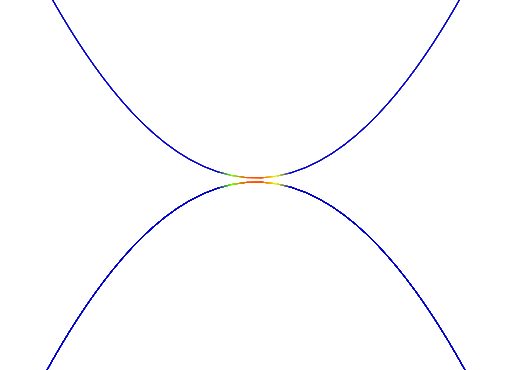
\includegraphics[width=.40\linewidth]{linearity-solution.png}};
    \spy on (0,.05) in node [left] at (2.2,1.7);
    \end{tikzpicture}
    \label{fig:linearity_solution}
}\\
\caption{Example of discontinuity in ambiguity from $\lambda$, with (b) and without (a) $\alpha$ modulation.}
\end{figure}

To address this, we define another modulating function $\alpha_{\mathbf{x}} : B(D(P)) \rightarrow [0,1]$ that smoothly weights the influence of paths on $\lambda$ as they approach $\mathbf{x}$. Specifically, $\alpha_{\mathbf{x}}$ smoothly decreases from 1 to 0 as the Euclidean distance between $\mathbf{x}$ and the closest point on $B(p_i) \in B(D(P))$ increases from 0 to $r$. Similar to $\beta_{\mathbf{x}}$, the specific formulation of $\alpha_{\mathbf{x}}$ is flexible, with Figure \ref{fig:alpha} showing its general shape, where the x-axis represent the distance from $p_i$ to $\mathbf{x}$.

Figure \ref{fig:linearity_solution} demonstrates the effect of applying $\alpha_{\mathbf{x}}$ to modulate $\lambda$. The visualization shows a smooth transition in ambiguity levels from high (red) through medium (yellow) to low (blue), confirming that the modulating function successfully eliminates the sharp discontinuities from the scalar field.

\begin{figure}[h]
\centering
\begin{tikzpicture}[scale=1.0]
\begin{axis}[
    axis x line = center,
    axis y line = left,
    x label style={at={(axis description cs:.5,-0.05)},anchor=north},
    y label style={at={(axis description cs:.05,.5)},rotate=0,anchor=south},
    xlabel = {Distance of path from $\mathbf{x}$},
    ylabel = {$\alpha_{\mathbf{x}}$},
    xtick={0},
    ytick={0, 0.5, 1.0},
    xmin=0, xmax=1.6,
    ymin=-0.15, ymax=1.1,
    trig format plots=rad,
]

\addplot [red, domain=0:1]{0.5*(1+cos(pi*x))}; 
\addplot [red, domain=1:\pgfkeysvalueof{/pgfplots/xmax}] {0}; 

\draw [dashed] (axis cs:1,\pgfkeysvalueof{/pgfplots/ymin}) -- (axis cs:1,\pgfkeysvalueof{/pgfplots/ymax});
\draw [thick, <->] (axis cs:0,-0.05) -- (axis cs:1,-0.05) node[pos=0.5, below] {$r$};

\end{axis}
\end{tikzpicture}
\caption{Graph with expected shape of $\alpha_{\mathbf{x}}$.}
\label{fig:alpha}
\end{figure}


With the modulating functions defined, we have a formulation for ambiguity given by $\gamma : \mathbb{R}^2 \rightarrow \mathbb{R}_{+}$, as follows:

\begin{equation}
\gamma(\mathbf{x} \in \mathbb{R}^2) = \sum_{p_i, p_j \in \bar{P}_{\mathbf{x}}}
\alpha_{\mathbf{x}}(p_i) \beta_{\mathbf{x}}(p_i) \lambda(p_i, p_j)
\end{equation}


% --- step 3:

\textbf{Convolution and normalization (steps 3 and 4):}
Given the scalar field defined by $\gamma$, we apply two final processing steps to optimize $\gamma$ for practical applications. While the modulating functions in $\gamma$ provide initial smoothness, we introduce a convolution step with an Epanechnikov kernel\cite{epanechnikov:1969} $K$ of radius $r$ to guarantee continuity across the entire field. This effectively eliminates potential discontinuities while preserving the essential characteristics of the ambiguity measure.

Following the convolution, we apply a normalization step to ensure field values remain in a consistent range. This normalization can be performed either relative to the existing maximum value in the scalar field, enabling in-dpeth comparison between regions of the same drawings, or through a limiting function, allowing cross-drawing comparisons. Given a user-defined paramter $c \in \mathbb{R}_{+}$, the limiting function is defined as follows:

% lucas: both the division by r^3 and the multiplication by 500 are to make the visualizations behave nicely when we change r. With this configuration, one might leave c at 1.0 and have generally good results across multiple r values. I don't know how to properly explain this in mathematical terms.
\begin{align}
t &= {\displaystyle \gamma(\mathbf{y}) \frac{500c}{r^3}}
\\
f(\mathbf{y} \in \mathbb{R}^2) &= 1 - \frac{1}{e^t}
\end{align}

By constraining $\gamma$ values, the limiting function makes bundle evaluation more stable and reliable when comparing different bundling techniques. This ensures that the scalar field can be used consistently to aid in bundle formation. To maintain visual consistency of the resulting bundles across varying $r$, the $\gamma$ is scaled by $500/r^3$. This scaling compensates for ambiguity growth with $r$, allowing for good visual results with $c = 1$ across different $r$ values.

Finally, we can define $\omega$ with the following equation:

\begin{equation}
\omega(\mathbf{x} \in \mathbb{R}^2) = \int_{\mathbf{y} \in \mathbb{R}^2}K(\|\mathbf{y} - \mathbf{x}\|)f(\mathbf{y})
\end{equation}

% ------- SUBSECTION -------

\subsection{Approximation Techniques}

Computing $\omega$ in real time presents significant challenges. Straightforward GPU implementations face two main issues. First is the compute time: calculating the distances for every pair of paths found throughout all $\bar{P}_p$ sets on-the-fly is computationally expensive. While this issue can be mitigated by pre-computing all pairwise distances, it comes at the cost of increased video memory (VRAM usage. The second issue is the high VRAM consumption required to store every $\bar{P}_p$ set of the drawing. In this case, the mitigations for the first issue clash directly with the second issue, as VRAM consumption quickly becomes too big for consumer hardware.

To address both of these issues, we developed an approximation approach that limits the size of the $\bar{P}_p$ sets by taking a random sub-sample. Our experiments indicate that limiting each set to a maximum of 100 paths preserves $\omega$ precision while drastically reducing VRAM consumption. This approach enables real-time calculation of $\omega$ on consumer-grade GPUs, with memory usage up to an order of magnitude lower compared to the non-approximated version. The random sub-sampling is performed using a simple reservoir sampling technique\cite{vitter:1985}.

% lucas: I have this almost ready from the qualification exam. Just needs to be adapted.
While this approximation introduces a slight trade-off between accuracy and memory efficiency, our experiments show that the impact on accuracy is negligible for most practical applications. The detailed validation for this approximation, including error analysis, can be found in the supplementary material.

% ------- SUBSECTION -------

\subsection{Validation}

Validating a new metric is always challenging, especially when there are no established standards for comparison. As discussed previously, $\omega$ introduces two novel contributions to ambiguity measurement: (1) local ambiguity values for the entire drawing instead of a single global value, and (2) a non-binary operator for crossing paths, where the ambiguity is modulated by the similarity of overlapping paths. Given this novel approach, we validate $\omega$ through a series of qualitative test cases with increasing complexity, demonstrating its effectiveness and reliability. All examples are of bundled drawings using the state-of-the-art CUBu framework\cite{van:2016}.

We begin with the simplest example: two pairs of connected clusters with a single crossing region, as demonstrated in Figure \ref{fig:validation_simple:straight}. In the bundled visualization (Figure \ref{fig:validation_simple:ambiguity}), tracing the original connectivity patterns of the clusters becomes impossible, as all paths converge into a single, ambiguous bundle in the center. This bundle obscures the original connections, creating ambiguity in the visualization. An effective ambiguity metric should reflect this situation by assigning higher values in the central bundle, where ambiguity is high, and lower values to areas where meaning is preserved. $\omega$ successfully captures this pattern, as seen in Figure \ref{fig:validation_simple:ambiguity}. Values are colored from blue (low ambiguity) to yellow (medium ambiguity) to red (high ambiguity), a scheme used consistently in all following test cases.

\begin{figure}[ht]
\centering
\subfloat[Input drawing]{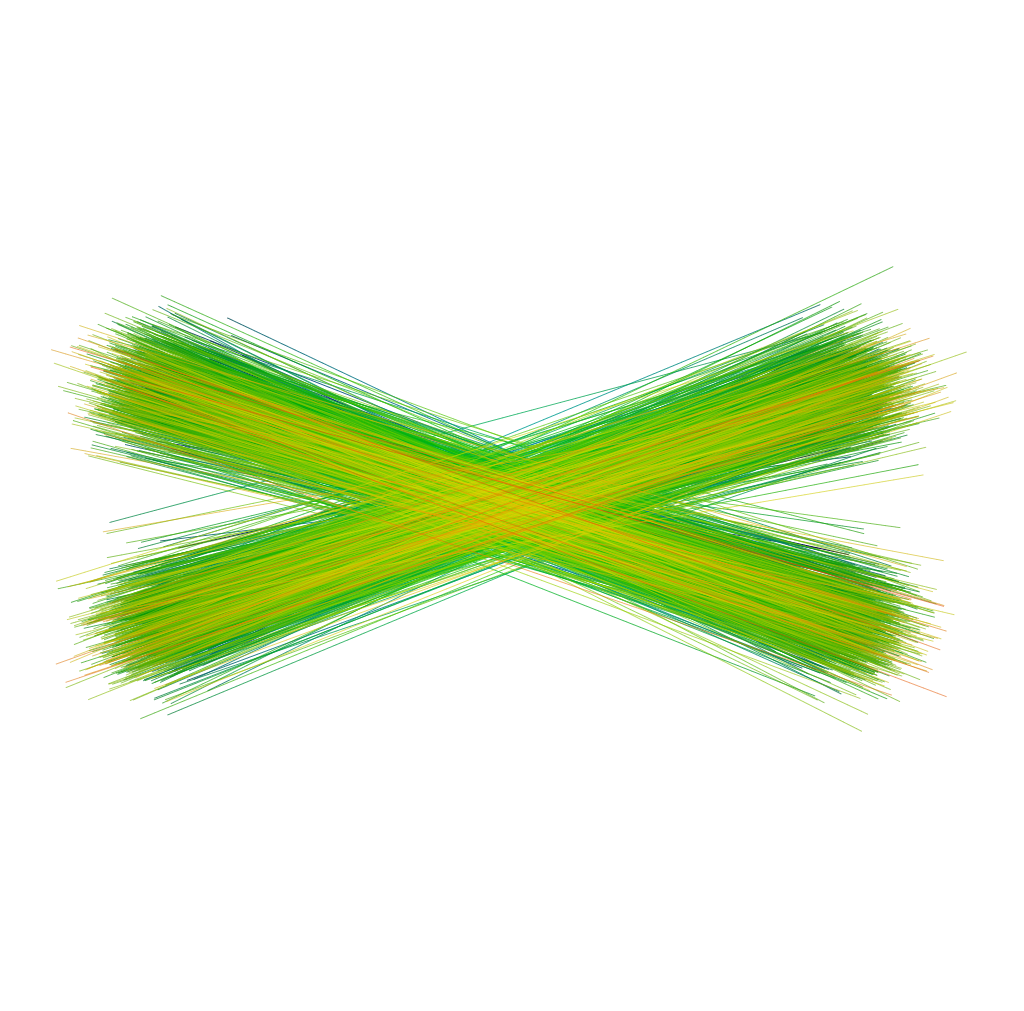
\includegraphics[width=0.48\linewidth]{metric_validation/1_straight.png}\label{fig:validation_simple:straight}}
\subfloat[Bundled drawing]{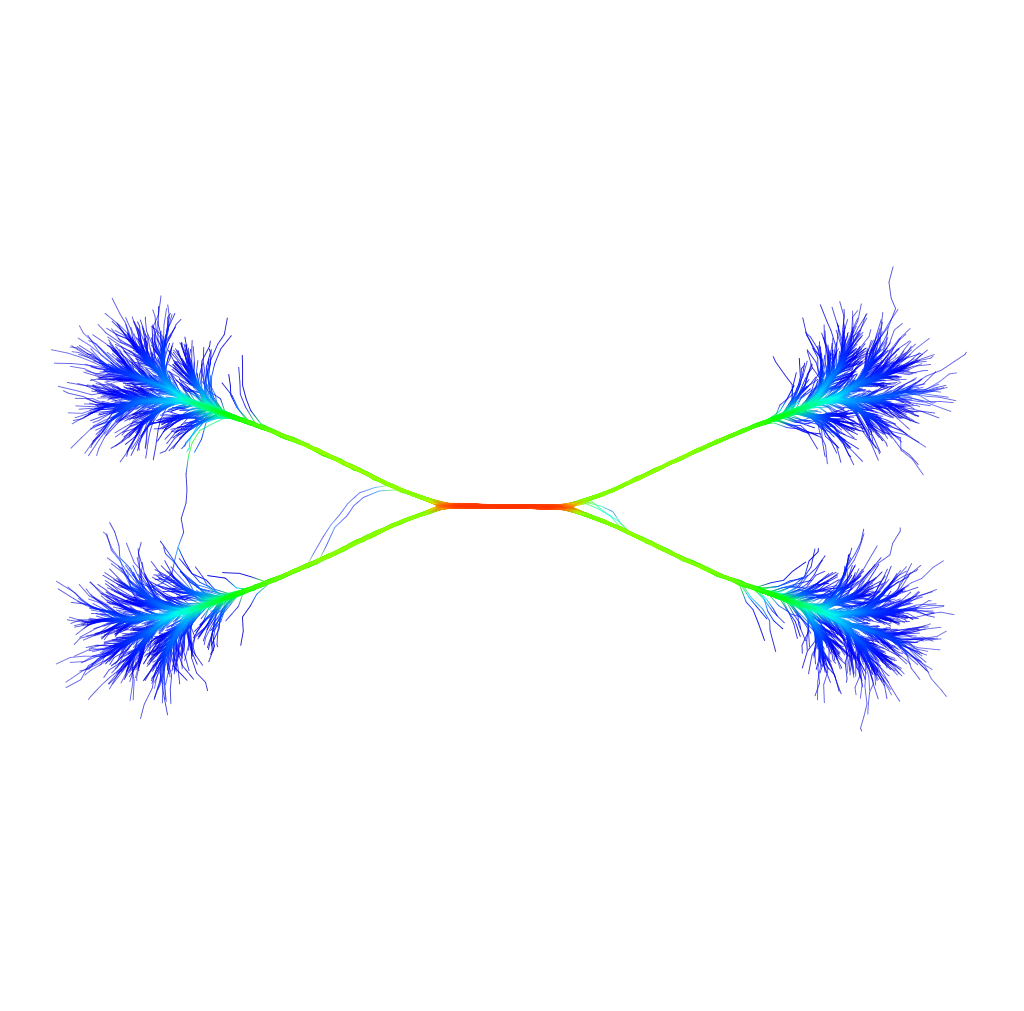
\includegraphics[width=0.48\linewidth]{metric_validation/1_bundled.png}\label{fig:validation_simple:ambiguity}}\\
\caption{Simple example of $\omega$ validation.}
\end{figure}

For a more complex example, we examine three pairs with three crossing regions, as depicted in Figure \ref{fig:validation_medium:straight}. Again, the bundled visualization (Figure \ref{fig:validation_medium:ambiguity}) obfuscates the connectivity patterns in the crossing regions, with multiple paths converging into the same bundle. However, this example introduces additional complexity through its crossing patterns. There are two ambiguous crossings and one non-ambiguous crossing, where the crossing is almost perpendicular. A robust ambiguity metric should correctly identify which of are the ambiguous crossings; which, as shown in Figure \ref{fig:validation_medium:ambiguity}, $\omega$ correctly does with the areas highlighted in red.

\begin{figure}[ht]
\centering
\subfloat[Input drawing]{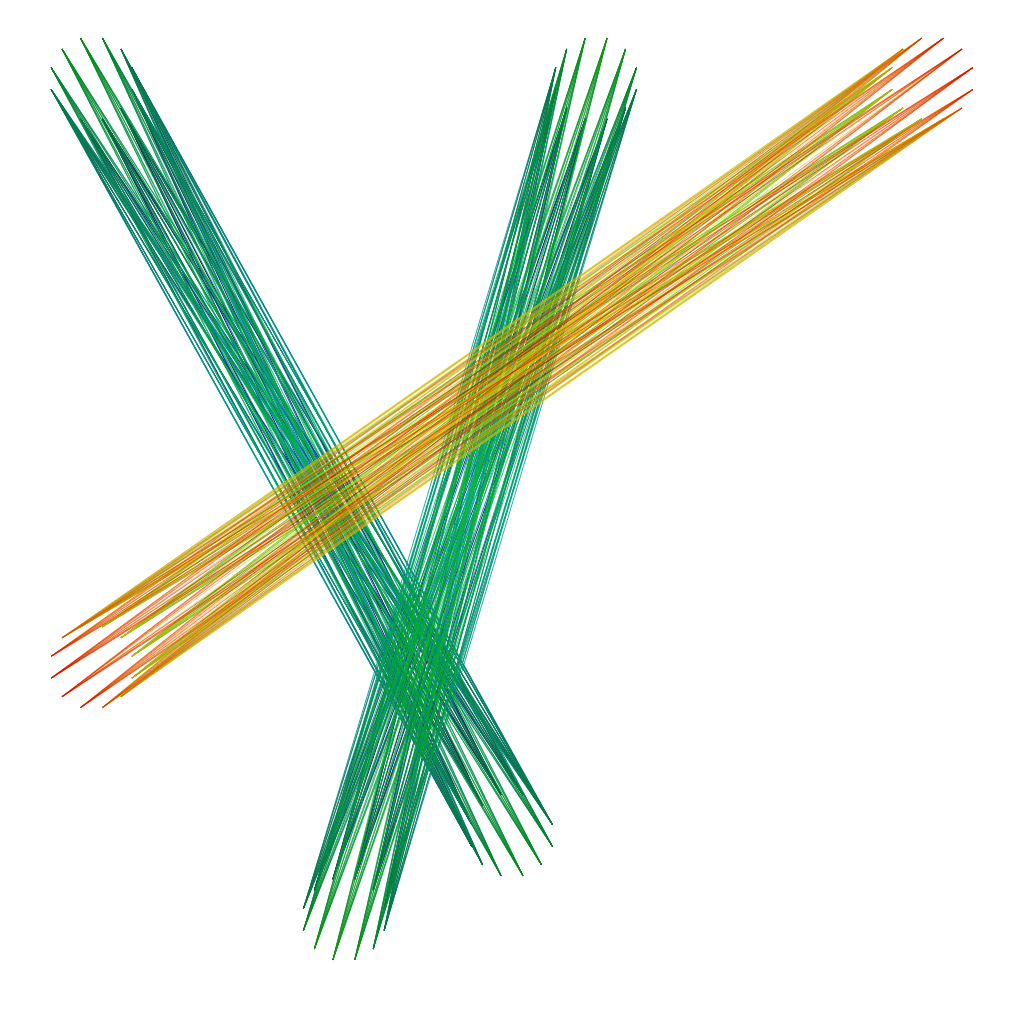
\includegraphics[width=0.48\linewidth]{metric_validation/2_straight.png}\label{fig:validation_medium:straight}}
\subfloat[Bundled drawing]{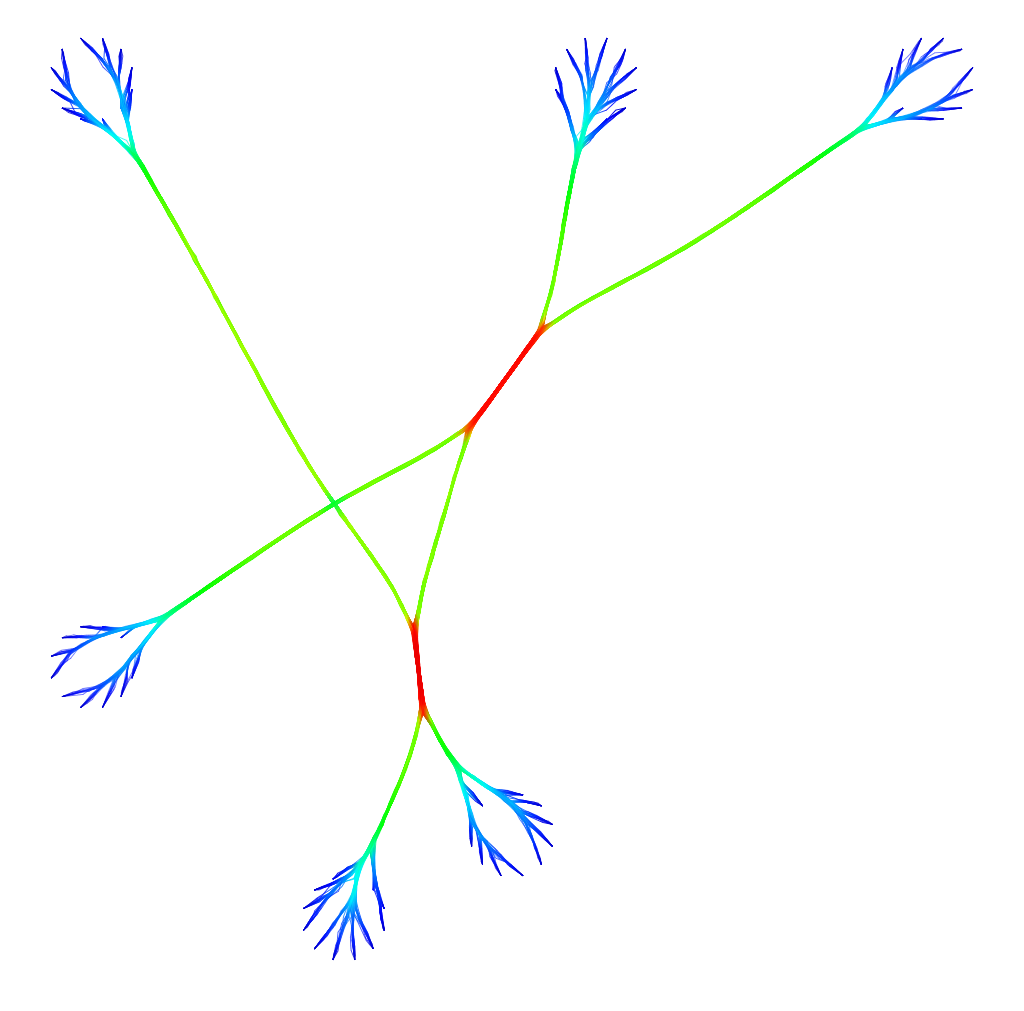
\includegraphics[width=0.48\linewidth]{metric_validation/2_bundled.png}\label{fig:validation_medium:ambiguity}}\\
\caption{Example of $\omega$ validation with perpendicular crossing paths.}
\end{figure}

For our next validation case, we examine when bundles overlap vertex clusters, as depicted in Figure \ref{fig:validation_overlap:straight}. In Figure \ref{fig:validation_overlap:ambiguity}, clusters are connected to multiple clusters instead of only one to one. Additionally, the bundles cross two of the central clusters. However, these overlaps should not be marked with high ambiguity, as it preserves the connectivity patterns of the original network. $\omega$ performs as expected, preserving low to medium ambiguity values in the mentioned bundles, while still highlighting as red the ambiguous cluster in the left side of Figure \ref{fig:validation_overlap:ambiguity}.

\begin{figure}[ht]
\centering
\subfloat[Input drawing]{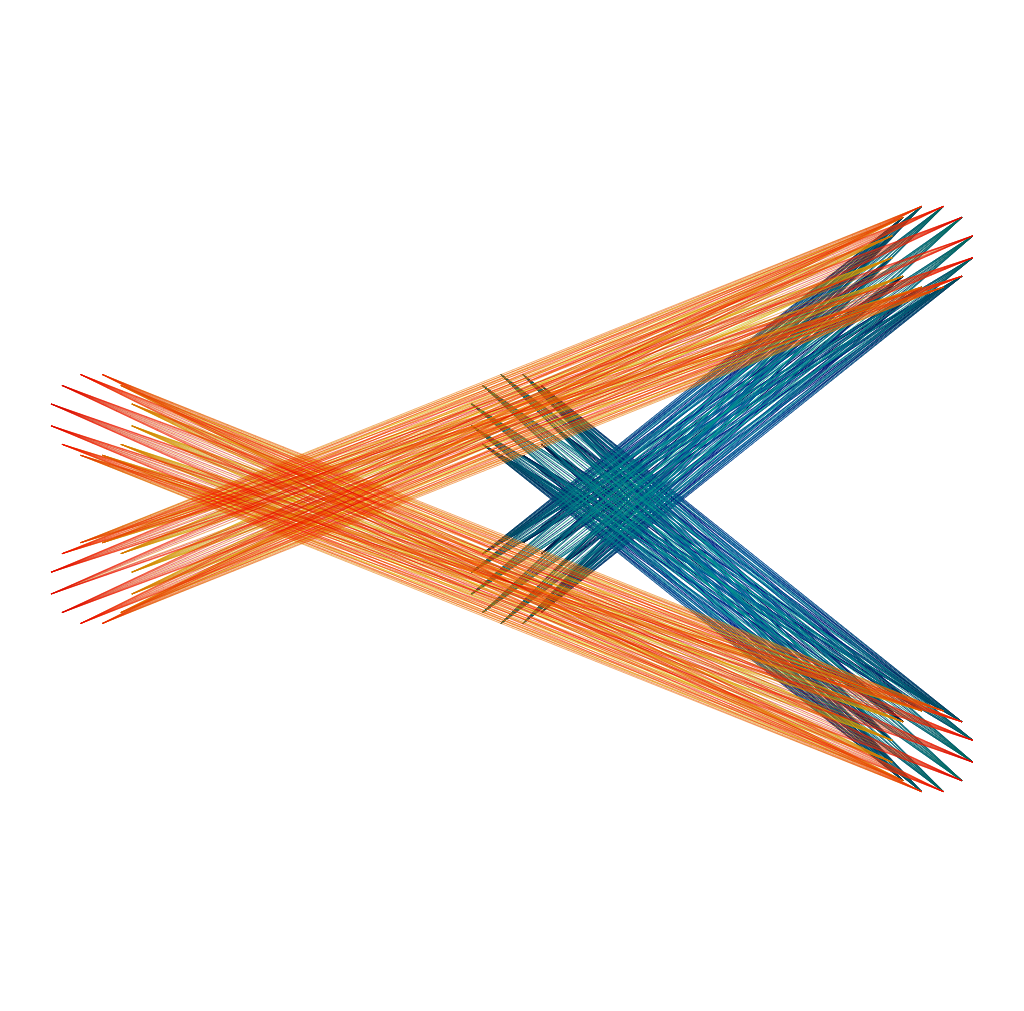
\includegraphics[width=0.48\linewidth]{metric_validation/3_straight.png}\label{fig:validation_overlap:straight}}
\subfloat[Bundled drawing]{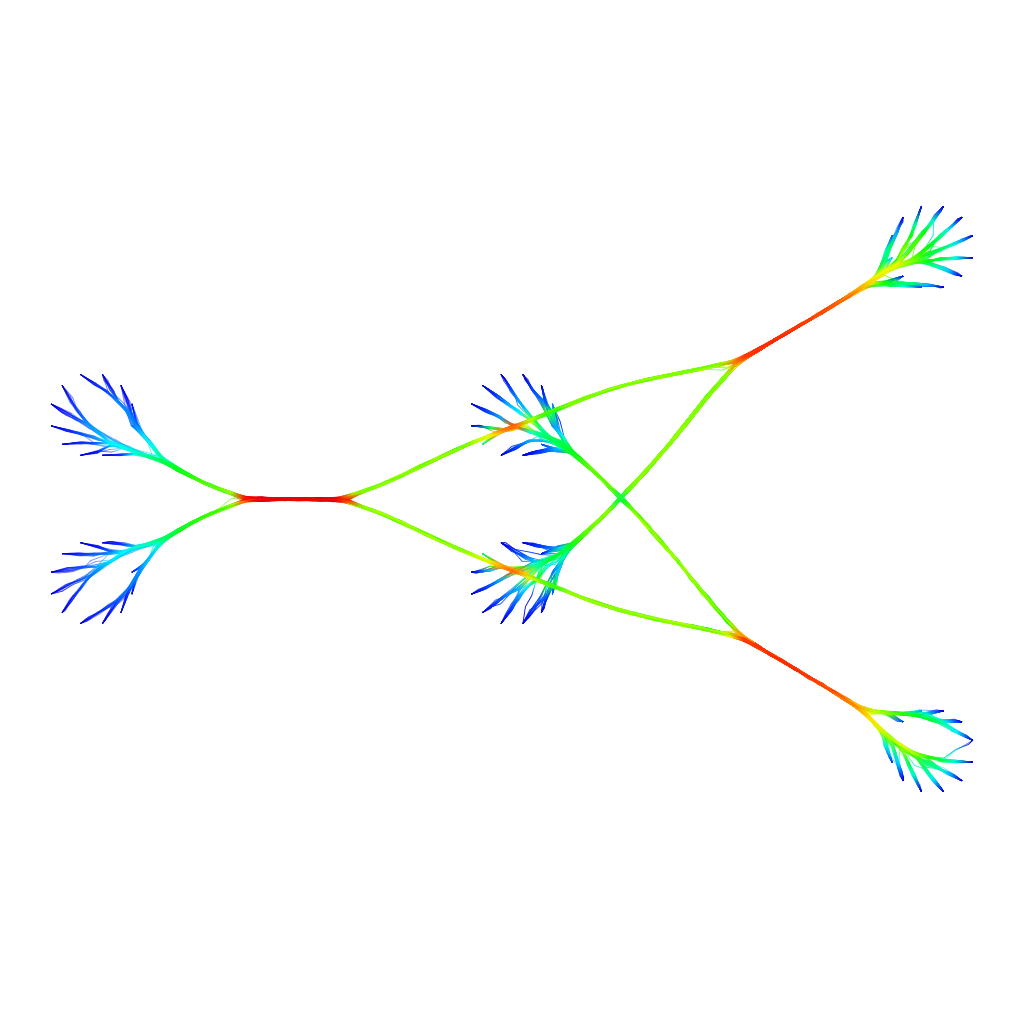
\includegraphics[width=0.48\linewidth]{metric_validation/3_bundled.png}\label{fig:validation_overlap:ambiguity}}\\
\caption{Example of $\omega$ validation with overlapping paths and endpoint clusters.}
\end{figure}

Finally, we consider a complex example with multiple ambiguous crossings and overlapping paths. Figure \ref{fig:validation_complex:straight} presents a network in the shape of a hexagon, where each cluster is connected to every other cluster. The bundled visualization (Figure \ref{fig:validation_complex:ambiguity}) creates a complex network of bundles, with multiple ambiguous crossings and overlapping paths. $\omega$ effectively captures this complexity, as shown in Figure \ref{fig:validation_complex:ambiguity}. Tracing bundles from each cluster, it is possible to see that every time divergent bundles meet, \textit{i.e.} where there is loss of perceived connectivity, $\omega$ assigns high ambiguity values to the region. The highlighted regions present examples of such ambiguous regions.

\begin{figure}[ht]
\centering
\subfloat[Input drawing]{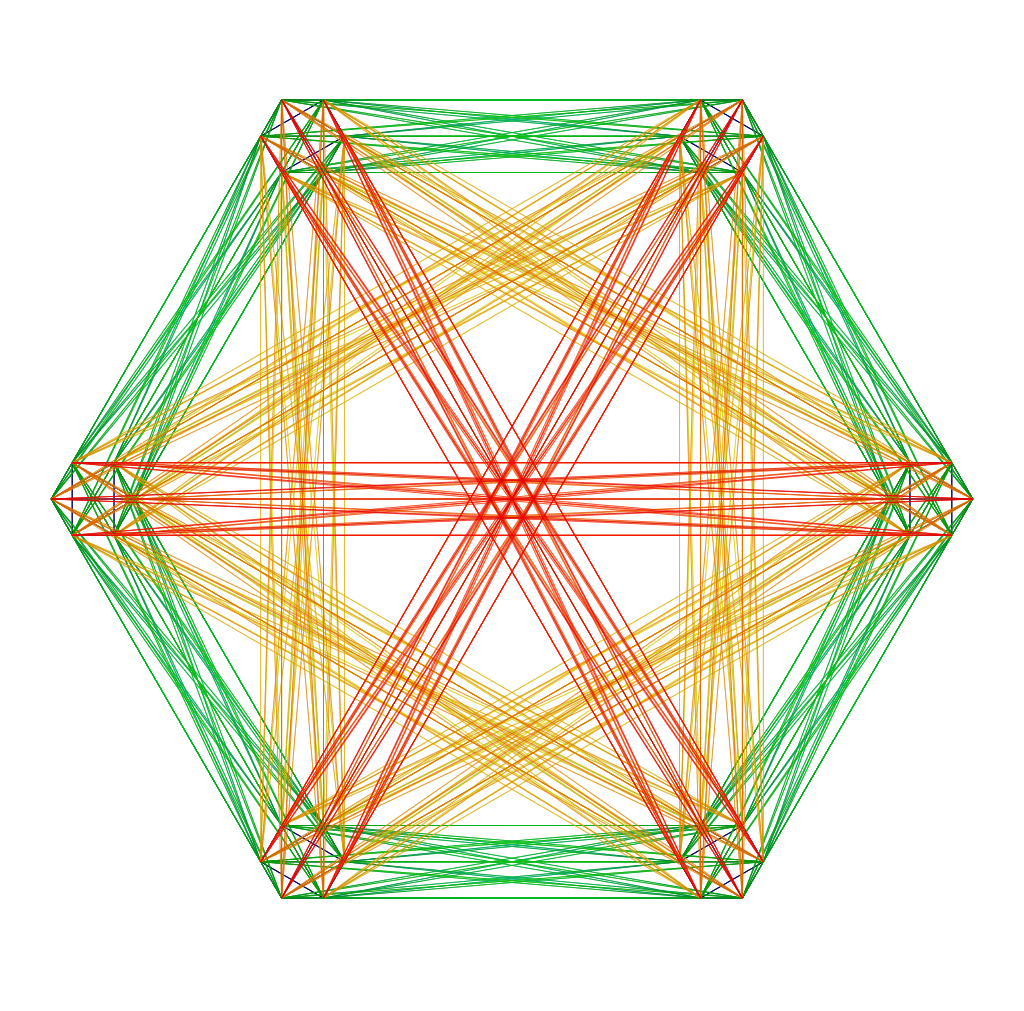
\includegraphics[width=0.48\linewidth]{metric_validation/4_straight.png}\label{fig:validation_complex:straight}}
\subfloat[Bundled drawing]{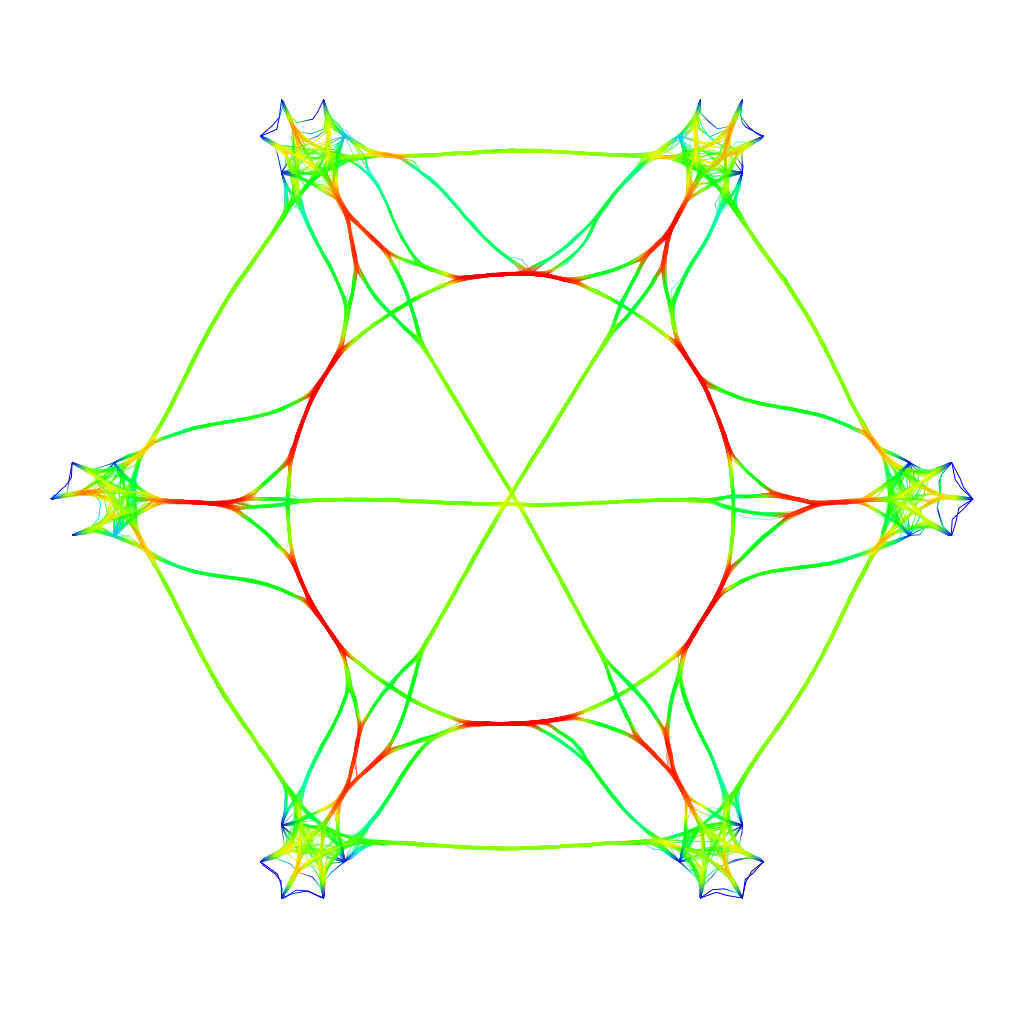
\includegraphics[width=0.48\linewidth]{metric_validation/4_bundled.png}\label{fig:validation_complex:ambiguity}}\\
\caption{Example of $\omega$ validation with complex data.}
\end{figure}


These validation cases demonstrate that $\omega$ successfully captures ambiguity patterns across a spectrum of complexity, from simple crossings to intricate bundling scenarios. The metric consistently identifies regions where connectivity information is compromised while appropriately handling cases where visual complexity does not necessarily imply ambiguity, such as bundle-cluster overlaps. Through these test cases, we have shown that $\omega$ fulfills its design goals: providing localized ambiguity measurements and accounting for path similarity in crossing regions. This validation establishes $\omega$ as a reliable tool for evaluating and potentially improving bundled graph visualizations.

% ------- SUBSECTION -------

\subsection{Parameters}

Our ambiguity metric presents three distinct parameters to customize the view of the user:

\begin{itemize}
\item $r \in \mathbb{N}$: This is the radius of neighborhood $N_r$ in step 1, and the radius of the convolution kernel in step 3. Lower values reduce the area of influence of ambiguous crossings, increasing the sharpness of the ambiguity map. Meanwhile, higher values increase the spread of ambiguity to neighbouring regions and smooth out the ambiguity values across the map. Typical values for $r$ range from 3 to 7. Figure \ref{fig:param_r} compares different values of $r$ with other parameters fixed.

\begin{figure}[ht]
\centering
\subfloat[$r = 3$]{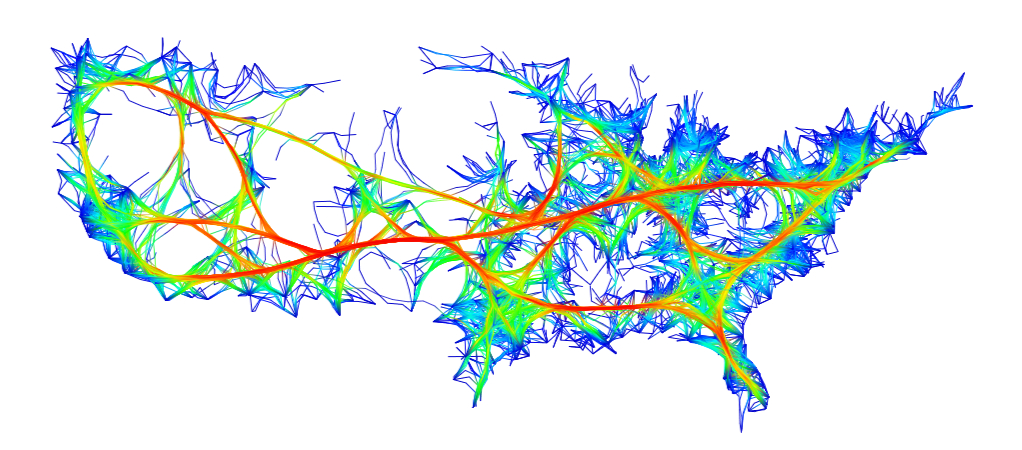
\includegraphics[width=0.48\linewidth]{params/r_3.png}}
\subfloat[$r = 5$]{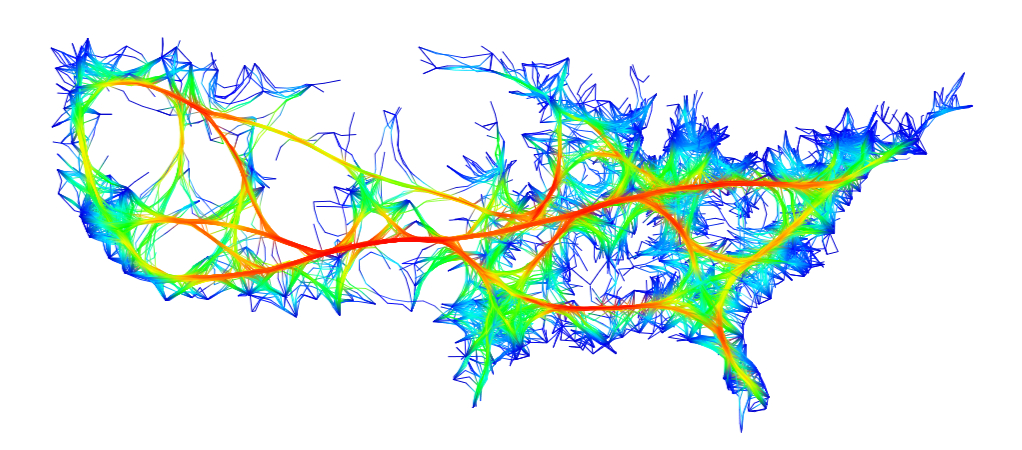
\includegraphics[width=0.48\linewidth]{params/r_5.png}}\\
\subfloat[$r = 7$]{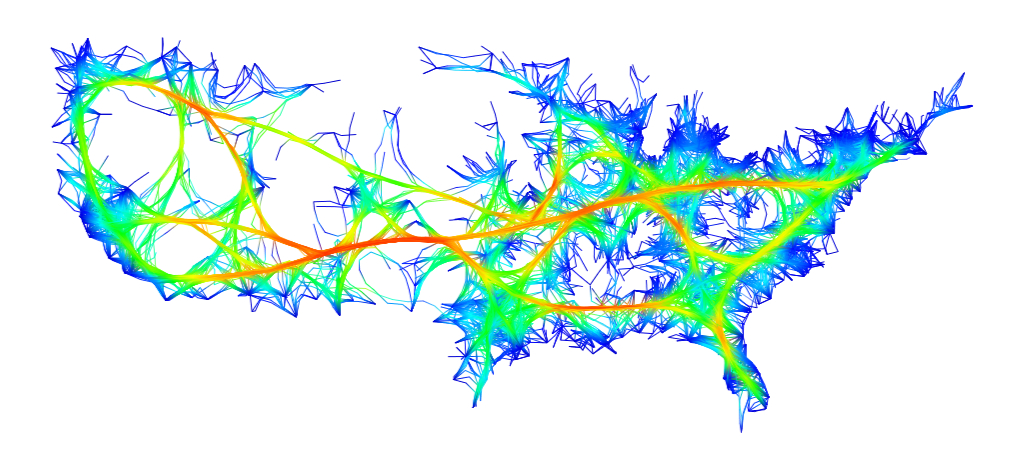
\includegraphics[width=0.48\linewidth]{params/r_7.png}}
\subfloat[$r = 9$]{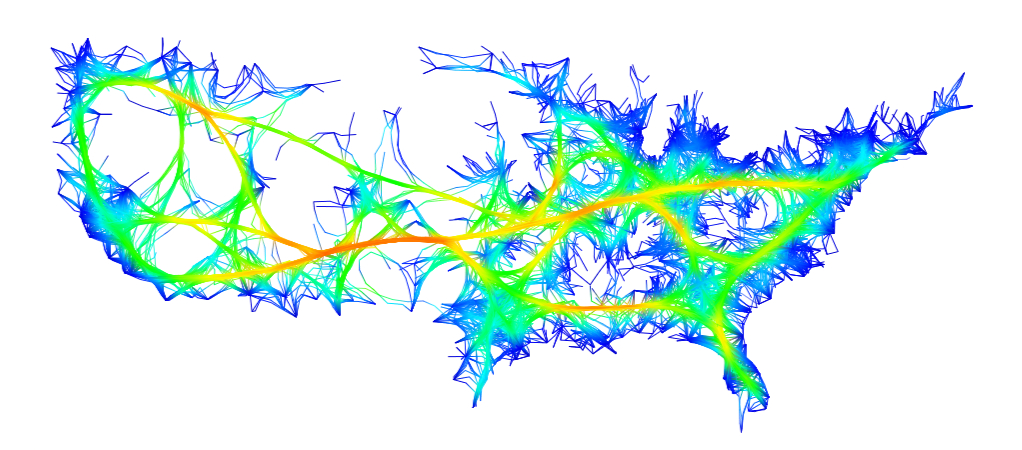
\includegraphics[width=0.48\linewidth]{params/r_9.png}}\\
\caption{Comparison of the same drawing with varying $r$ and all other parameters fixed.}
\label{fig:param_r}
\end{figure}

\item $m \in [0, 0.5]$: This controls the modulation of ambiguity values of paths according to their distance from path endpoints, described in-depth in step 2. Lower values decrease the distance to which values are modulated, while higher values increase it. A $m$ value of 0.25 provides a good middle ground for the general case. Figure \ref{fig:param_m} compares different values of $m$ with other parameters fixed.

\begin{figure}[ht]
\centering
\subfloat[$m = 0$]{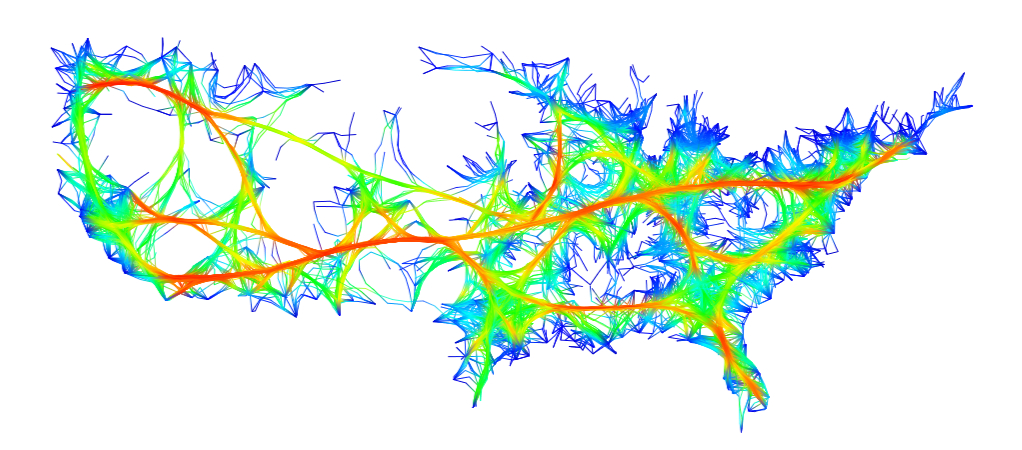
\includegraphics[width=0.48\linewidth]{params/m_.00.png}}
\subfloat[$m = 0.25$]{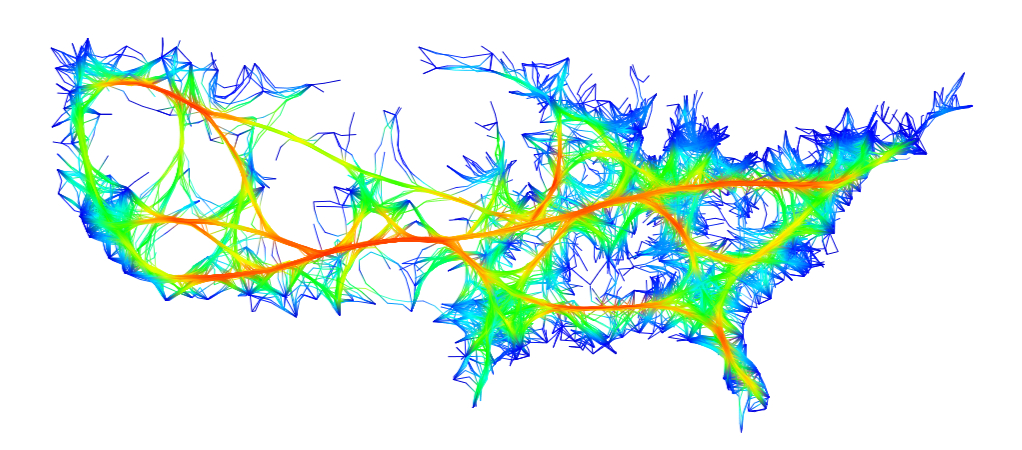
\includegraphics[width=0.48\linewidth]{params/m_.25.png}}\\
\subfloat[$m = 0.50$]{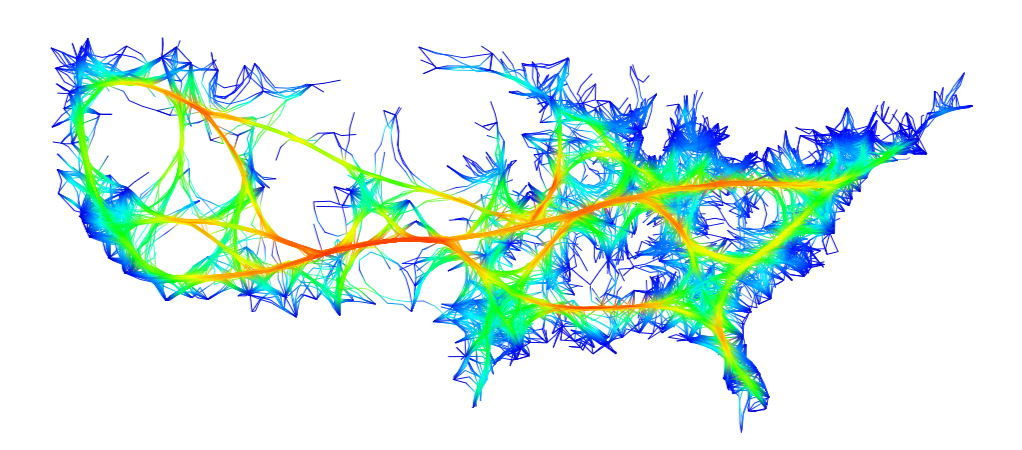
\includegraphics[width=0.48\linewidth]{params/m_.50.png}}
\subfloat[$m = 0.75$]{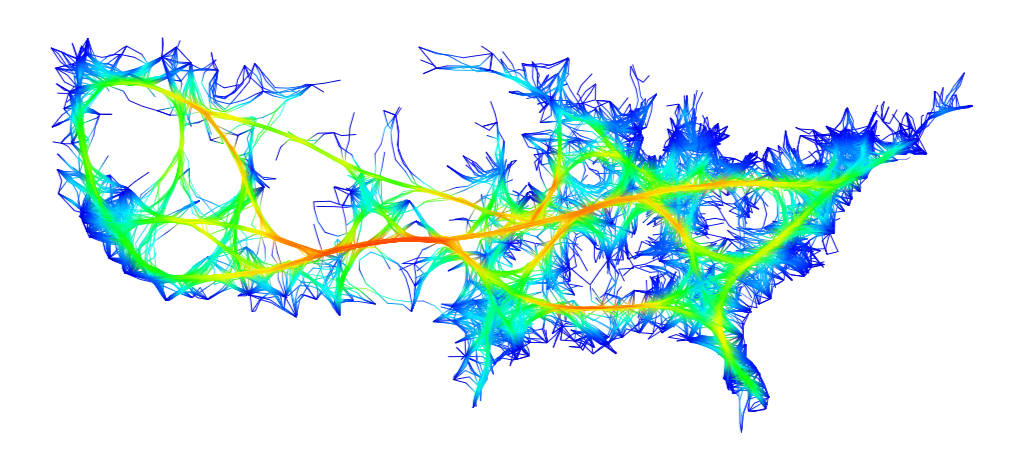
\includegraphics[width=0.48\linewidth]{params/m_.75.png}}\\
\caption{Comparison of the same drawing with varying $m$ and all other parameters fixed.}
\label{fig:param_m}
\end{figure}

\item $c \in \mathbb{R}_{+}$: This defines the threshold used to normalize the ambiguity values across the map, as described in step 4. Lower values will be more sensitive to ambiguity, presenting higher final values from lower raw ambiguity values. The opposite holds for higher values of $c$. As we adjust $c$ according $r$, a good all-round value for $c$ is 1. Figure \ref{fig:param_m} compares different values of $c$ with other parameters fixed.

\begin{figure}[ht]
\centering
\subfloat[$c = 0.6$]{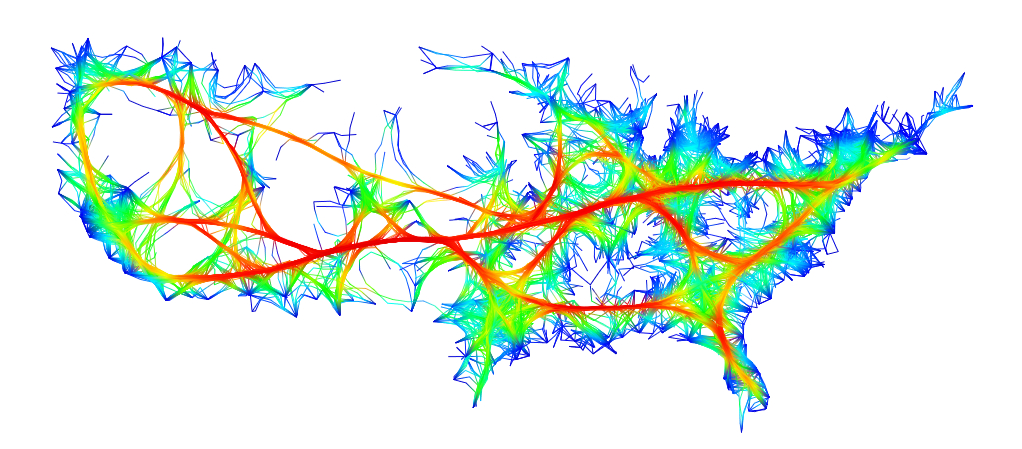
\includegraphics[width=0.48\linewidth]{params/c_0.6.png}}
\subfloat[$c = 0.8$]{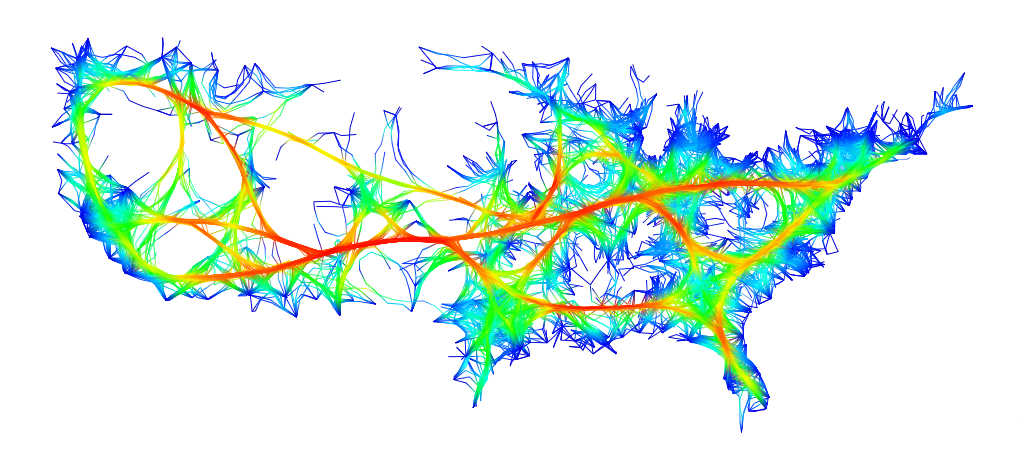
\includegraphics[width=0.48\linewidth]{params/c_0.8.png}}\\
\subfloat[$c = 1.0$]{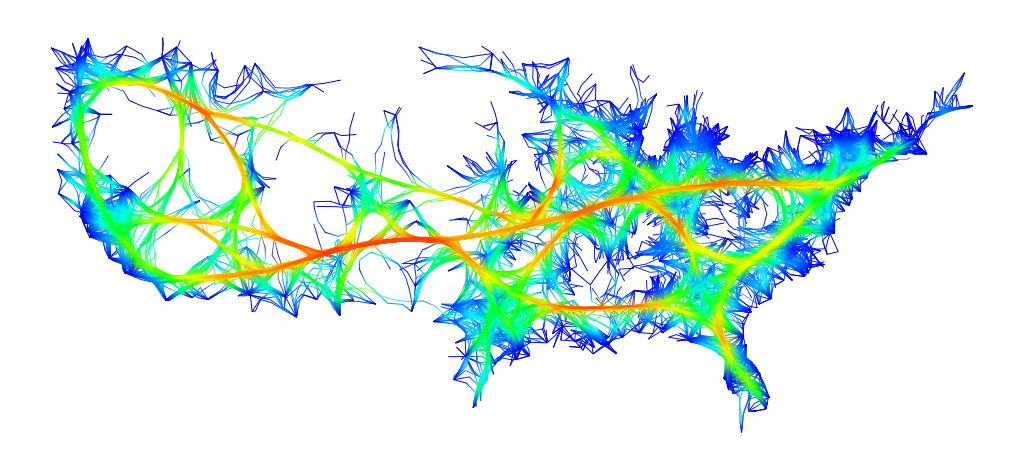
\includegraphics[width=0.48\linewidth]{params/c_1.0.png}}
\subfloat[$c = 1.2$]{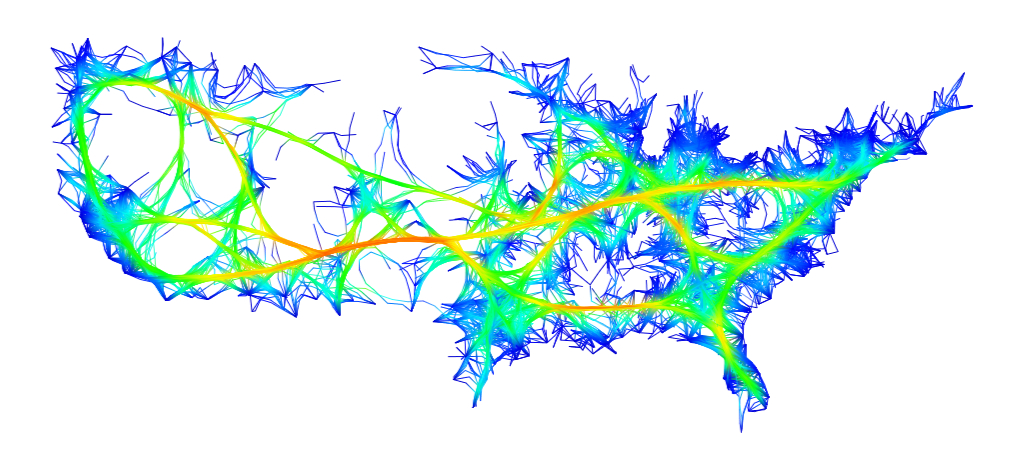
\includegraphics[width=0.48\linewidth]{params/c_1.2.png}}\\
\caption{Comparison of the same drawing with varying $m$ and all other parameters fixed.}
\label{fig:param_m}
\end{figure}

\end{itemize}
